\section{User Manual}
Source code and build scripts for the \mw\ with a name server and the client implementation exists at two locations:

\begin{tabular}{l}
	$\sim$\texttt{/c10mjn/edu/5dv147/project/}\\
	$\sim$\texttt{/c12slm/edu/5dv147/project/}\\
\end{tabular}

Where source code exists in the \texttt{src/} directory. The source code can also be cloned from our git repository with:

\begin{verbatim}
git clone https://github.com/Minty-Tnaeg/GCOM_middleware.git
\end{verbatim}

Please note the entire project is built in Java 1.8.

\subsection{Build \& Run}
The client and \mw\ and the name server all exists in the same executable \texttt{jar} that can be compiled with a \textit{ant} displayed below. The script will give a client executable and an example is shown below.

\begin{verbatim}
ant client
\end{verbatim}

The name server exists in the same directory and is built with the same \textit{ant} script but has a different argument and is displayed below. The script will generate a executable \texttt{jar} that will register a name server service for the machine running the program. 

\begin{verbatim}
ant server
\end{verbatim}

\subsection{Name Server}
The name server will start a \textit{rmiregistry} on the machine running the \textit{jar} on port $33401$, where clients may connect. If the server succeeds with starting the program will print.

\begin{verbatim}
Name Server started
\end{verbatim}

To start with help of the \textit{jar} use the following command line:
\begin{verbatim}
java -jar GCOM_server.jar
\end{verbatim}


\subsection{Client}
The client is started after the build with the help of:
\begin{verbatim}
java -jar GCOM_client.jar
\end{verbatim}

When the client starts it will give a window where the user has to supply a alias used for chatting, a address to the name server and the name servers port and enable/disable debug mode.
If the server then is available a group list window will be displayed where the user may supply a group name and will join if the name exists or create a new if the name is free. 

If the user then joins a group it will give a chat window and if debug was enabled it will also produce a frame for the logical clock and other settings for the debugging of the client.

% Show figure of settings window
\begin{figure}[h!]
\centering
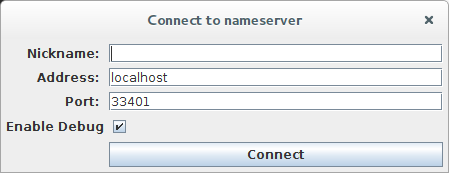
\includegraphics[width=0.6\textwidth]{Pictures/login}
\caption{Start-window for the program. Allows input of Nameserver information, your own nickname as well as choosing wether to use debug or not. }
\end{figure}

% Show figure of group list
\begin{figure}[h!]
\centering
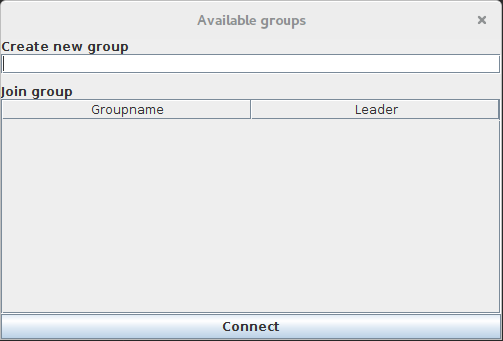
\includegraphics[width=0.6\textwidth]{Pictures/groupChoose}
\caption{Window for choosing which group to join. Also allows creation of new groups. }
\end{figure}

% Show figure of chat window
\begin{figure}[h!]
\centering
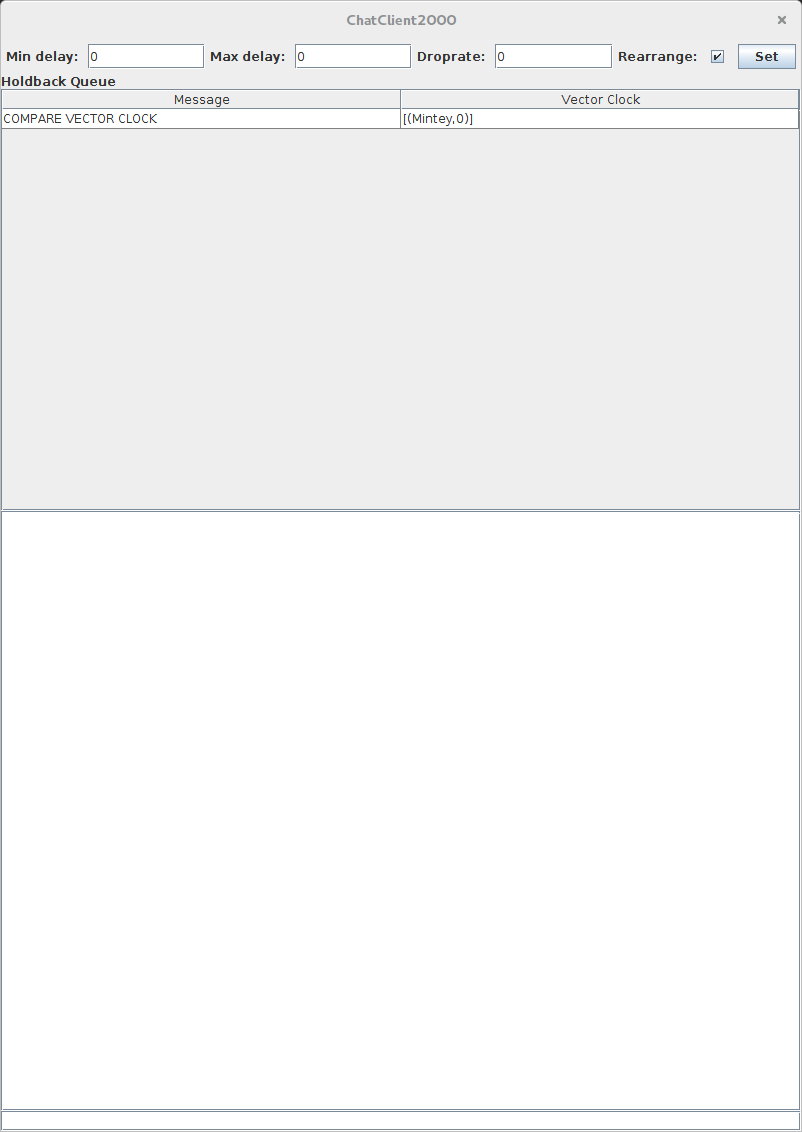
\includegraphics[width=0.7\textwidth]{Pictures/debugAndChat}
\caption{The first window shows all current messages in the hold-back queue as well as choose debug settings. The second window is the chat-window which will display all delivered messages and allow you to send your own. }
\end{figure}

\pagebreak
